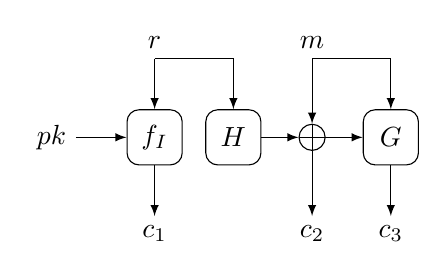
\begin{tikzpicture}
\node (f1) [rounded corners=1ex,minimum size=0.7cm, draw] {$f_{I}$};
\node (h1) [right of=f1, node distance=1cm, minimum size=0.7cm, rounded corners=1ex, draw] {$H$};
\node (p1) [right of=h1, node distance=1cm, circle, radius=0.5cm, draw] {};
\draw[-] (p1.north) -- (p1.south);
\draw[-] (p1.east) -- (p1.west);
\node (g1) [right of=p1, node distance=1cm, minimum size=0.7cm, rounded corners=1ex, draw] {$G$};


\draw[-latex] (0,1cm) node [above] {$r$} -- (f1);
\draw[-latex] (0,1cm) -| (h1.north);
\draw[-latex] (2,1cm) node [above] {$m$} -- (p1);
\draw[-latex] (2,1cm) -| (g1);
\draw[-latex] (-1cm,0) node [left] {$pk$} -- (f1);
\draw[-latex] (h1) -- (p1.west);
\draw[-latex] (f1) -- +(0,-1) node [below] {$c_1$};
\draw[-latex] (p1) -- +(0,-1) node [below] {$c_2$};
\draw[-latex] (p1) -- (g1);
\draw[-latex] (g1) -- +(0,-1) node [below] {$c_3$};
\end{tikzpicture}